\documentclass[11pt]{article}
\usepackage[paper=letterpaper, left=1in, right=1in, top=1in, bottom=1in]
           {geometry}
\usepackage[parfill]{parskip}
\usepackage{amsmath}

\usepackage{mathtools}
\DeclarePairedDelimiter\ceil{\lceil}{\rceil}
\DeclarePairedDelimiter\floor{\lfloor}{\rfloor}
\usepackage{graphicx}
\usepackage{fancyvrb}
\usepackage{upquote}
\usepackage[en-GB]{datetime2}
\DTMlangsetup[en-GB]{ord=omit}
\usepackage{xfrac}

\newcommand{\answer}{\textit{Analysis: } }


\begin{document}
\thispagestyle{empty}

\begin{center}
{\large CS 310}\\
\textbf{Assignment 0911 - Algorithm Analysis}
\end{center}

\begin{flushright}
Bill Jin
\end{flushright}

\section*{Analysis for push function:}

1.\textbf{push} function code $\colon$

\begin{Verbatim}[numbers=left,xleftmargin=5mm]
void push(unsigned element)
{
  heap.push_back(element);
  bubble_up(heap.size() - 1);  
}
\end{Verbatim}

2.\textbf{bubble\_up} function code $\colon$
\begin{Verbatim}[numbers=left,xleftmargin=5mm]
void bubble_up(size_t position)
{
  if (position != 0)
  {
    size_t parent = (position - 1) / 2;
    while (position != 0 && heap.at(position) > heap.at(parent))
    {
      std::swap(heap.at(position), heap.at(parent));
      position = parent;
      parent = (position - 1) / 2;
    }
  }
}
\end{Verbatim}

\answer This algorithm is used to place the node into its right place by using while loop swapping its parent node with if the node is greater than that. And for the input size will be the size of the heap we build.

For the \textbf{worst cases} (Big-O), the operations that are counted are:

In push function $\colon$
\begin{itemize}
\item the push\_back function, count as 1 operation,
\end{itemize}

In bubble\_up function $\colon$
\begin{itemize}
\item the if condition comparison on line 3, count as 1 operation,
\item the assignment of parent, count as 1 operation,
\item while loop condition, since it has 3 comparisons, count as $\floor{ \log_2(n+1)} \times 3$ operations,
\item swap function, count as $\floor{ \log_2(n+1)} \times 2$ operations,
\item assignment of position, count as $\floor{ \log_2(n+1)} \times 1$ operations,
\item parent assignment on line 10, count as $\floor{ \log_2(n+1)} \times 1$ operations,
\item one more for loop condition check, count as $\floor{ \log_2(n+1)} \times 3$ operations.
\end{itemize}

After sum up all, the number of times of all operations that are executed is$\colon$

\[
 \floor{ \log_2(n+1)} \times 10 + 3
\]

For the \textbf{best cases} (Big-$\Omega$), the operations that are counted are:

In push function $\colon$
\begin{itemize}
\item the push\_back function, count as 1 operation.
\end{itemize}

In bubble\_up function $\colon$
\begin{itemize}
\item we assume it only has root which means only run if condition, count as 1 operation.
\end{itemize}

After sum up all, the number of times of all operations that are executed is :
\[
\text{2 operations}
\]

Since there are while loop and if conditions which could cause the best and the worst cases. Therefore, we can find out that this algorithm belongs to Big-Oh and Big-Omega efficiency class.
\[
    T(n) \in O(\log_2(n)) \text{ for $c$ = 10, all $n$ $\geq$ 0}    
\]

\[
    T(n) \in \Omega(1)
\]

And the resulting data file is plotted, we get the following. Also
plotted on the same axes are the scaled standard functions $ \log_2(n+1) \times 10 + 3$ and
2 which illustrate that the algorithm belongs to big-O and big-$\Omega$ .

\begin{center}
  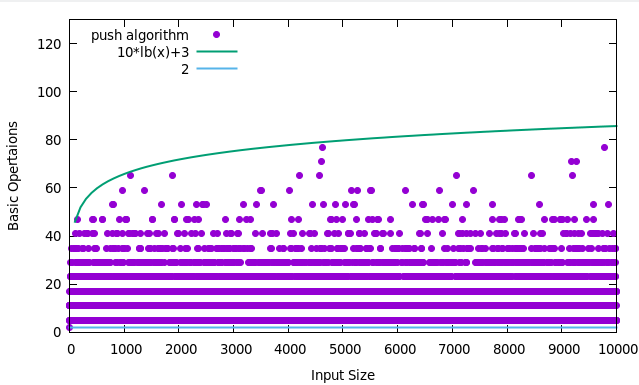
\includegraphics[width=0.7\textwidth]{push_function.png}
\end{center}
\newpage


\section*{Analysis for pop function:}
1.\textbf{pop} function code $\colon$

\begin{Verbatim}[numbers=left,xleftmargin=5mm]
unsigned pop()
{
  assert(heap.size() > 0);
  unsigned value_to_return = heap.at(0);
  heap.at(0) = heap.at(heap.size() - 1);
  heap.pop_back();    
  percolate_down(0);
  return value_to_return;
}
\end{Verbatim}

2.\textbf{percolate\_down} function code $\colon$
\begin{Verbatim}[numbers=left,xleftmargin=5mm]
void percolate_down(size_t position)
{
  size_t left_child_position;
  size_t right_child_position;
  
  left_child_position = 2 * position + 1;
  right_child_position = 2 * position + 2;

  bool loop_guard = true;
  
  while (number_of_chidren(position) >= 1 && loop_guard)
  {
    if (number_of_chidren(position) == 2)
    {
      if (heap.at(left_child_position) <= heap.at(right_child_position))
      {
        if (heap.at(position) <= heap.at(right_child_position))
        {
          std::swap(heap.at(position), heap.at(right_child_position));
          position = right_child_position;
        }
        else
        {
          loop_guard = false;
        }
      }
      else
      {  
        if (heap.at(position) <= heap.at(left_child_position))
        {
          std::swap(heap.at(position), heap.at(left_child_position));
          position = left_child_position;
        }
        else
        {
          loop_guard = false;
        }
      }
    }
    else if (number_of_chidren(position) == 1) 
    {
      if (heap.at(position) < heap.at(left_child_position))
      {
        std::swap(heap.at(position), heap.at(left_child_position));
        position = left_child_position;
      }
      else
      {
        loop_guard = false;
      }
    }
    left_child_position = 2 * position + 1;
    right_child_position = 2 * position + 2;
  }
  ((void)0);
}
\end{Verbatim}

\answer This algorithm is used to put the node into its right place by using while loop swapping its children node with. And for the input size will be the size of the heap we build.

For the \textbf{worst cases} (Big-O), the operations that are counted are:

1. \textbf{pop function} $\colon$
\begin{itemize}
\item the assert function, count as 1 operation,
\item value\_to\_return assignment count as 1 operation,
\item assignment of root node, count as 1 operation,
\item heap.pop function, count as 1 operation,
\item return value, count as 1 operation.
\end{itemize}

2. \textbf{percolate\_down function} $\colon$
\begin{itemize}
\item two children declarations and assignment from line 3 to 7, count as 4 operations,
\item loop\_guard declaration assignment, count as 1 operation,
\item while condition, count as $\floor{ \log_2(n+1)} \times 2$ operations, 
\item if condition for worst case, count for $\floor{ \log_2(n+1)} \times 1$ operation,
\item next if condition on line 17, count for $\floor{ \log_2(n+1)} \times 1$ operation,
\item swap function on line 19, count as $\floor{ \log_2(n+1)} \times 2$ operations,
\item else if condition check, count as $\floor{ \log_2(n+1)} \times 1$ operation,
\item both left and right side children assignments, count as $\floor{ \log_2(n+1)} \times 2$ operations
\item while loop count one more time, count as $\floor{ \log_2(n+1)} \times 2$ operations
\end{itemize}

After sum up all, the number of times of all operations that are executed is$\colon$
\[
 \floor{ \log_2(n+1)} \times 11 + 10
\]

For the \textbf{best cases} (Big-$\Omega$), the operations that are counted are:

1. \textbf{pop function} $\colon$
\begin{itemize}
\item the assert function, count as 1 operation,
\item value\_to\_return assignment count as 1 operation,
\item assignment of root node, count as 1 operation,
\item heap.pop function, count as 1 operation,
\item return value, count as 1 operation.
\end{itemize}

2. \textbf{percolate\_down function} $\colon$
\begin{itemize}
\item two children declarations and assignment from line 3 to 7, count as 4 operations,
\item loop\_guard declaration assignment, count as 1 operation,
\item heap only has one node, the root, so while loop will not run, count only the condition 2 operations.
\end{itemize}

After sum up all, the number of times of all operations that are executed is$\colon$
\[
\text{6 operations}
\]

Since there are while loop and if conditions which could cause the best and the worst cases. Therefore, we can find out that this algorithm belongs to Big-Oh and Big-Omega efficiency class.
\[
    T(n) \in O(\log_2(n)) \text{ for c = 11, all n $\geq$ 1}    
\]

\[
    T(n) \in \Omega(1)
\]

And the resulting data file is plotted, we get the following. Also
plotted on the same axes are the scaled standard functions $ \log_2(n+1) \times 11 + 10$ and
6 which illustrate that the algorithm belongs to big-O and big-$\Omega$ .

\begin{center}
  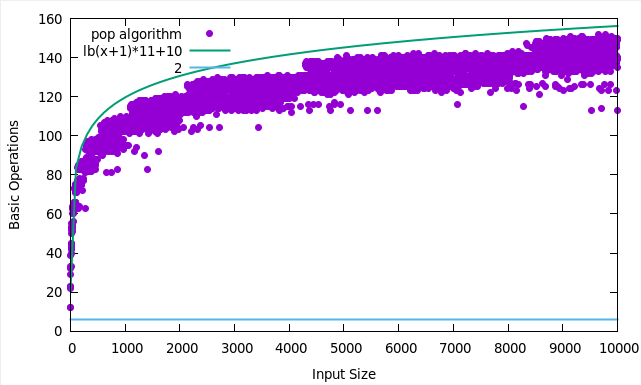
\includegraphics[width=0.7\textwidth]{pop_function.png}
\end{center}
\newpage

\end{document}


